\section{Classifier Evaluation}
\subsection{Confusion Matrix}
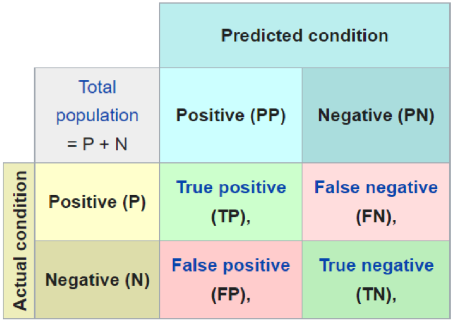
\includegraphics[width=0.8\linewidth]{confusion_matrix-1.png}

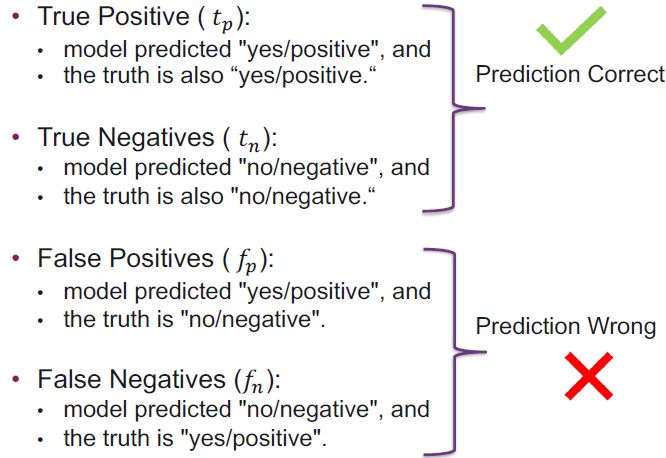
\includegraphics[width=0.8\linewidth]{confusion_matrix-2.png} \\

\textbf{Mean Accuracy}
\begin{itemize}
    \item How often is the classifier correct?
    \item $A = (t_p + t_n) / n$
\end{itemize}
\vspace{10pt}
\textbf{Mean Error}
\begin{itemize}
    \item How often is the classifier wrong?
    \item $E = (f_p + f_n) / n$
\end{itemize}
\vspace{10pt}
\textbf{Precision}
\begin{itemize}
    \item When the prediction is 1, how often is it correct?
    \item $P = t_p / (t_p + f_p)$
\end{itemize}
\vspace{10pt}
\textbf{Sensitivity, Recall, True Positive Rate (TPR)}
\begin{itemize}
    \item How often the prediction is 1 when it's actually 1
    \item $R = t_p / (t_p + f_n)$
\end{itemize}
\vspace{10pt}
\textbf{Miss Rate, False Negative Rate (FNR)}
\begin{itemize}
    \item $MR = 1 - TPR$
\end{itemize}

\subsubsection{Why Accuracy is not enough?}
\begin{itemize}
    \item If the prediction is constant the accuracy may still look decent
    \item E.g. always predict false
    \item 90\% of the data is false
    \item Accuracy = 90\% (decent)
    \item Precision = 0
    \item Recall = 0
\end{itemize}

\subsection{Precision vs. Recall}
\begin{itemize}
    \item Increasing precision reduces Recall and vice versa
    \item Threshold is a business decision (depending on goals)
\end{itemize}
\vspace{10pt}
\textbf{Examples}
\begin{itemize}
    \item \textcolor{blue}{Classify videos safe for kids} Low recall (rejects many safe videos), high precision (keeps only safe ones)
    \item \textcolor{blue}{Classify shoplifters from a surveillance camera} Low precision but high recall (false alerts are ok)
\end{itemize}

\subsection{Receiver Operating Characteristics (ROC)}
Verwende unterschiedliche Werte für den \textcolor{blue}{Threshold}, konvertiere die predicted Wahrscheinlichkeit zu Predicted Classes \\

\begin{itemize}
    \item Unterschiedliche Threshold resultieren in unterschiedlichen TPR und FPR
    \item Defined by FPR and TPR as x and y axes
    \item Visualizes tradeoff between TP (benefits) and FP (cost)
\end{itemize}
\begin{center}
    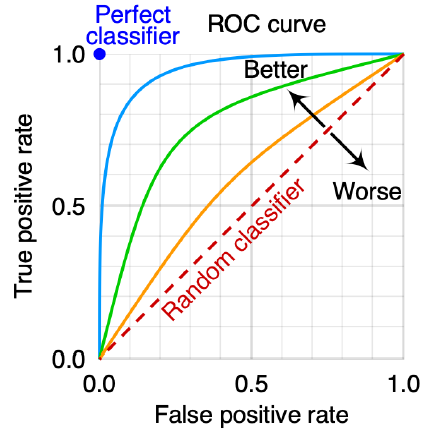
\includegraphics[width=0.7\linewidth]{roc.png}
    Plot mit Kurve von TPR vs. FPR für verschiedene Thresholds
\end{center}
\vspace{10pt}
\textbf{Area under the curve}
\begin{itemize}
    \item Shows how well the TPR and FPR is looking in the aggregate
    \item The greater the area under the curve, the higher the quality of the model
    \item The greater the area, the higher the ratio of true positives (TP) to false positives (FP)
\end{itemize}
